\subsection{Power filtrations}

Finally, we move to our last construction of a filtered simplicial complex. The typical road-map for computation of persistent homology is to take a point cloud in some metric space, construct a filtered Vietoris-Rips complex, and then compute the persistent homology of the complex. In this subsection, we explore an alternative filtered simplicial complex we may construct from graphs that we may apply persistent homology to. Some applications of such a construction can be found in Chapter \ref{cha:applications}. Many of the definitions here are taken from the work by \textcite{ferri2018simplicial}.

\begin{definition}[Graph]
    A \emph{undirected graph} is a tuple $G = (V,E)$ where $V$ is a set of objects called \emph{vertices} and $E \subset \{\{x,y\}: x,y \in V, x \neq y\}$ is a set of \emph{edges}.
\end{definition}

This is a traditional definition of a graph, but we can simply view it as a $1$-simplicial complex where the vertices are the $0$-simplices and the edges are $1$-simplices. The above definition may be referred to as an \emph{undirected simple graph}. A directed graph may be similarly defined where the vertices in the edges are ordered (resembling ordered simplices), and a simple graph is one with no self loops (that is, $\{x\} \not\in E$) and no two vertices may have more than one edge between them.

\begin{definition}
    Let $G = (V,E)$ be an undirected graph.
    \begin{enumerate}
        \item (\emph{Adjacency}) The vertices in an edge may be referred to as \emph{endpoints}, and two points are \emph{adjacent} if there exists an edge between them.
        \item (\emph{Paths and cycles}) A \emph{path} in a graph is a ordered collection of vertices such that there is an edge between any two adjacent vertices. A \emph{path} is called a \emph{cycle} if the first and last vertex coincide. The \emph{length} of a path $p = (v_1, \ldots, v_n)$ is $\lvert p \rvert = n-1$.
        \item (\emph{Subgraphs}) Let $G = (V,E)$ and $G' = (V', E')$ be graphs. $G'$ is a \emph{subgraph} of $G$ if $V' \subset V$ and $E' \subset E$.
        \item (\emph{Induced subgraphs}) Let $S \subset V$. Then the subgraph \emph{induced by $S$}, denoted $G[S]$, is the graph whose vertex set is $S$ and whose edge set consists of all edges in $E$ that have both endpoints in $S$.
        \item (\emph{Neighbourhoods}) The \emph{neighbourhood} of a vertex $v \in V$ is the subgraph of $G$ induced by all vertices adjacent to $v$. 
        \item (\emph{Graph metric}) We may impart a graph with a metric, define
        \begin{align*}
            d: V \times V & \to \mathbb N_0 \cup \{\infty\},                             \\
            d(u,v)        & = \min\{p: \text{$p$ is a path from $u$ to $v$}\}.
        \end{align*}
        If $u = v$, then define $d(u,v) = 0$. If no such path from $u$ to $v$ exists, then define $d(u,v) = \infty$. From this, we derive a sense of the size of a graph: define the \emph{diameter} of $G$ as
        \[ \diam(G) = \max_{(u,v) \in V^2} d(u,v). \]
        \item (\emph{Graph power}) Define the \emph{$k$th power} $G^k$ of $G$ as
        \[ G^k = \left(V, \left\{\{u, v\} \subset V: 1 \leq d(u,v) \leq k \right\}\right). \]
        See Figure \ref{fig:power-graph} for an example of the powers of a small graph. 
        \item (\emph{Clique}) $G$ is said to be a \emph{clique} if every two distinct vertices are adjacent. Alternatively, if $\diam G = 1$. 
    \end{enumerate}
\end{definition}

For a graph $G$, we may sometimes denote the set of vertices of $G$ by $V(G)$, and the set of edges of $G$ by $E(G)$. 

\begin{figure}
    \makebox[\textwidth][c]{
      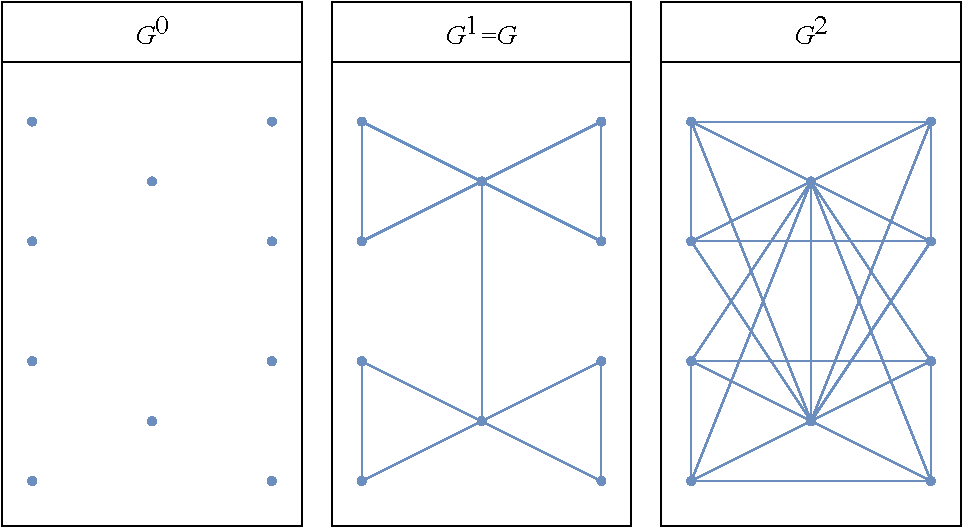
\includegraphics[width=0.8\textwidth]{content/2-background/images/power-graph}
    }
    \caption{An example of $G^k$ for $k \in \{0,1,2\}$, for a small 10-vertex graph $G$.}
    \label{fig:power-graph}
  \end{figure}

\begin{definition}[Clique complex]
    Let $G = (V,E)$ be an undirected graph. The \emph{clique complex} of $G$ is defined as
    \[ \Cl(G) = \left\{ S \subset V: \text{$G[S]$ is a clique} \right\}. \]
\end{definition}

Since every subset of a clique is itself a clique, $\Cl(G)$ is well-defined. The clique complex of a graph simply \emph{fills in} higher dimensional simplices for which all faces are present.

\begin{definition}[Power filtration]
    Let $G = (V,E)$ be an undirected graph. Define the \emph{power filtration} $\Pow(G)$ of $G$ as the filtration
    \[ \Pow(G): \Cl(G^0) \subset \Cl(G^1) \subset \ldots \subset \Cl(G^{\diam G}). \]
\end{definition}

The power filtration of a graph is a commonly used construction for applying persistent homology.

We will later make use of the \emph{Jaccard index}, which gives us a notion of how \emph{similar} two nodes are, based on their neighbourhoods. 

\begin{definition}[Jaccard index]
    Let $G = (V,E)$ be an undirected graph. The \emph{Jaccard index} $J: V^2 \to [0,1]$ is defined by
    \[ J(u,v) = \frac{\lvert V(N(u)) \cap V(N(v)) \rvert}{\lvert V(N(u)) \cup V(N(v)) \rvert}. \]
\end{definition}

If two nodes $u, v \in V$ share the same neighbours, then $J(u,v) = 1$. Conversely, if two nodes share no neighbours, then $J(u, v) = 0$. 



% We introduce some common simplicial complexes that may be built from a graph $G = (V,E)$, as described in \cite{ferri2018simplicial}.

% \begin{description}
%     \item[Clique complex $X(G)$] Consider every $(p+1)$-clique of $G$ as an abstract $p$-simplex.
%     \item[Independence complex $I(G)$] Consider every $(p+1)$-independent set of $G$ as an abstract $p$-simplex.
%     \item[Neighborhood complex $N(G)$] For every $v \in V$, consider the generating simplex $\{x\} \cup \{y \in V: \text{$y$ is adjacent to $x$}\}$.
%     \item[Induced acyclic subset complex $A(G)$] A non-zero set of vertices is a simplex if its induced graph is acyclic.
% \end{description}

% These complexes serve as an introduction to how simplicial complexes may be built from graphs, but we move to a more involved construction. We aim towards a construction that allows persistent homology to provide insight into the structure of the graph.

% \begin{definition}
% \end{definition}

% \texttt{todo}